\subsection{Параметры декодера}\label{subsec:arch}

Для достижения максимального качества работы декодера выполнен поиск оптимальных гиперпараметров. Проведен анализ результатов поиска и выбран набор параметров $s^*$, определенный в \ref{subsec:opt_hyper}.

Ниже представлен пошаговый процесс реализации нейронной сети $\mathcal{N}$ с параметрами $s^*$.

\begin{figure}[h]
    \centering
    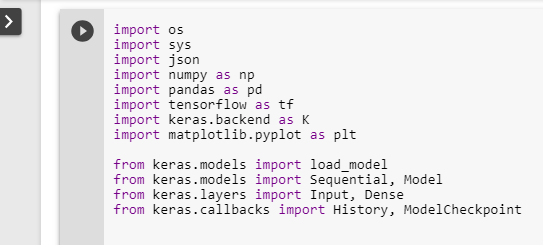
\includegraphics[width=0.9\textwidth]{neural_network_import.png}
    \caption{Импорт необходимых библиотек.}
    \label{fig:neural_network_import}
\end{figure}

\begin{figure}[h]
    \centering
    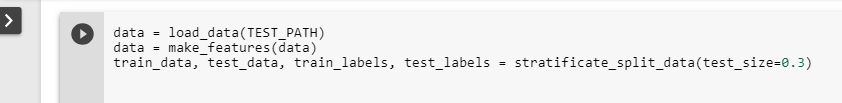
\includegraphics[width=0.9\textwidth]{neural_network_load.png}
    \caption{Загрузка и разделение данных.}
    \label{fig:neural_network_import}
\end{figure}


\begin{figure}[h]
    \centering
    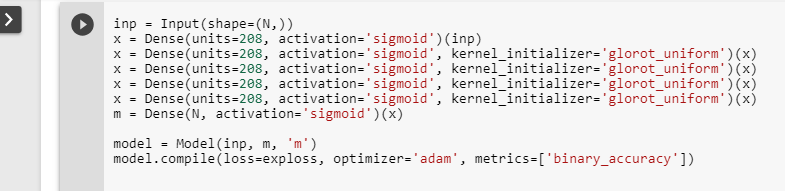
\includegraphics[width=0.9\textwidth]{neural_network_create.png}
    \caption{Создание модели нейронной сети.}
    \label{fig:neural_network_create}
\end{figure}

\newpage

\begin{figure}[h]
    \centering
    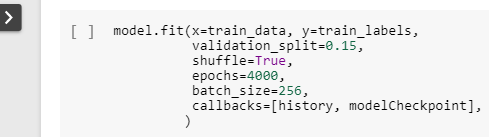
\includegraphics[width=0.9\textwidth]{neural_network_fit.png}
    \caption{Обучение модели.}
    \label{fig:neural_network_fir}
\end{figure}
